\documentclass[oneside, 12pt]{article}

\newcommand{\source}[1]{\textbf{Source:} {#1} }

\usepackage{indentfirst}
\usepackage{listings}
\usepackage{graphicx}
\usepackage{float}
\usepackage{color}
\usepackage{amsmath}
\usepackage[utf8]{inputenc}
\usepackage[english]{babel}
\usepackage[backend=bibtex]{biblatex}
\usepackage{color}
\usepackage{appendix}

\addbibresource{ref.bib}

\definecolor{pblue}{rgb}{0.13,0.13,1}
\definecolor{pgreen}{rgb}{0,0.5,0}
\definecolor{pred}{rgb}{0.9,0,0}
\definecolor{pgrey}{rgb}{0.46,0.45,0.48}

\usepackage{listings}
\lstset{language=Java,
  showspaces=false,
  showtabs=false,
  breaklines=true,
  showstringspaces=false,
  breakatwhitespace=true,
  commentstyle=\color{pgreen},
  keywordstyle=\color{pblue},
  stringstyle=\color{pred},
  basicstyle=\ttfamily,
  moredelim=[il][\textcolor{pgrey}]{\$\$},
  moredelim=[is][\textcolor{pgrey}]{\%\%}{\%\%}
}

\begin{document}
\title{Java 8 Parallel Streams}
\author{Ethan Williams}
\date{\today}
\maketitle

\tableofcontents

\setcounter{section}{-1}
\section{Prerequisites}

\subsection{Technical}
This document was written for Java developers who have an interest in using concurrency in streams, and assumes knowledge of serial streams and lambda expressions. Developers in other languages with similar mechanisms such as C\# with \verb|Linq| may also find the topics useful with the understanding that syntax, implementation, and functionality will differ.

Additionally, functional knowledge of \verb|java.util.concurrent| and the \verb|Consumer| interface will help in gaining a more practical knowledge but is not required.

\subsection{Vocabulary Clarification} \label{language}
Some of the vocabulary in the paper may be unfamiliar to those with a knowledge of streams and are defined/clarified below:
\begin{itemize}
\item A stream instantiated with the \verb|stream()| method only is referred to as a \textit{serial stream}
\item A stream instantiated with the \verb|parallel().stream()| or \verb|parallelStream()| methods is referred to as a \textit{parallel stream}
\item \textit{Serializing data} refers to destroying the stream and bringing all collection items left in the stream into memory
\item A stream is composed of 3 parts: a source which is the \verb|Collection| it is operating on, intermediate operations such as \verb|map()| which don't serialize data, and terminal operations like \verb|toArray()| which serialize the stream
\end{itemize}

\section{Introduction}
Parallel streams were introduced into Java 8 alongside serial streams so that developers could utilize concurrency in order to more efficiently utilize modern multiprocessor design \autocite{ibm_streams}. In the case of parallel streams, each thread handles a different part of the stream and assemble all the parts together when the stream is serialized \autocite{parallelism_doc}

Making a serial stream into a parallel stream is as easy as calling \verb|parallel()| after \verb|stream()|. In order for the \verb|parallel()| method to be applicable on the stream, the \verb|Collection| must have an implementation of a \verb|Spliterator| \autocite{ibm_streams}, an object which can effectively break up a collection to be processed separately. 

Several operations are more essential to parallel streams, as is the case with \verb|Collector|s. Calling the \verb|collect()| method on the stream will reduce and serialize it based on the behavior of the \verb|Collector| object passed as an argument \autocite{collector_doc}. With parallel streams, \verb|Collector|s are the recommended strategy for reduction because other mechanisms that can be used in serial streams will result in inconsistent results when run in parallel. The reason for this is discussed in Section \ref{stateful_expressions}.

Despite parallel streams being introduced into Java to simplify concurrency, developers can easily corrupt data and cause system bugs. All possible bugs in streams derive from developers not following standard concurrency practices such as using long-running or blocking operations in streams. Additionally, considerations have to be taken with streams specifically to avoid interference with the source and using stateful expressions.

\section{Spliterator}
{\itshape \verb|Spliterator| implementations differ based on the type of source collection, so this section focuses on a modified implementation for Java's \verb|ArrayList|}.
\newline

The \verb|Spliterator| is the backbone of parallel streams, allowing the program to split a collection apart (illustrated in Figure \ref{fig:split}) and iterate through it. If a class extending a \verb|Collection| does not have a \verb|spliterator()| method returning a \verb|Spliterator| object, then Java is not able to process the collection with a parallel stream at all. In many implementations including the one used in this paper, each instance has a source collection, an index, and a fence. The backing collection for each instance is the entire collection it is based on which ensures every instance has a consistent copy of the source. The index is the current cursor position of the \verb|Spliterator|, which is analogous to the cursor position in an \verb|Iterator| object. The fence is the index of the last element the Spliterator is responsible for plus one.

\begin{figure}[H]
\centering
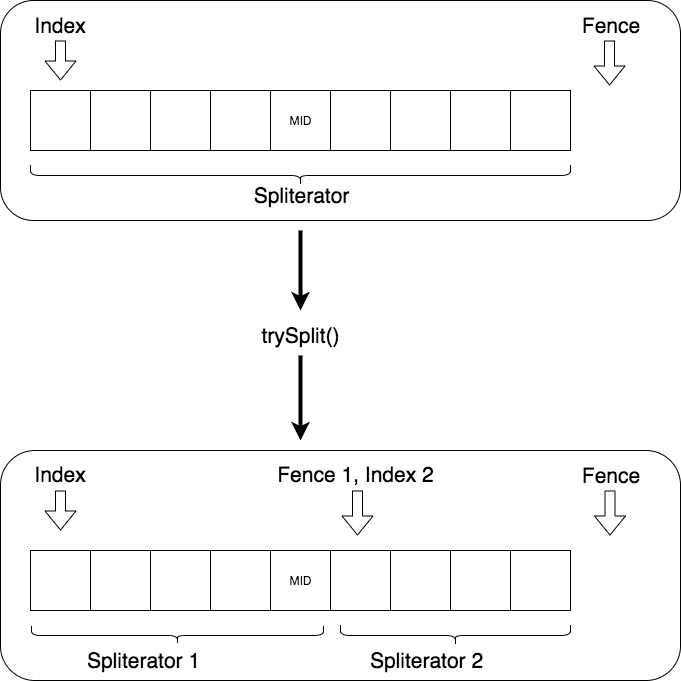
\includegraphics[width=8cm]{images/spliterator_illustrated.png}
\caption{A Spliterator Before and After Splitting}
\source{Ethan Williams}
\label{fig:split}
\end{figure}

\subsection{Implementation} 
Although the cursor is similar to \verb|Iterator|'s, traversal through a Spliterator using \verb|tryEachRemaining()| and \verb|tryNext()| is different. \verb|tryEachRemaining()| in Figure \ref{fig:forEachRemaining} takes a Consumer object which is the operation to be executed on each element of the collection. A typical implementation will simply iterate through all elements and call the \verb|accept()| method on the consumer with the element as its only parameter. \verb|tryNext()| in Figure \ref{fig:tryAdvance} is similar although the operation is only attempted on element at the current cursor position. If that cursor position is past the fence of the Spliterator, then the method returns false, otherwise it returns true.

\begin{figure}[H]
\centering
\begin{lstlisting}[language=Java]
public void forEachRemaining(Consumer<? super E> action) {
    int i;
    if ((i = index) >= 0 && (index = fence) <= a.length) {
        for (; i < hi; ++i)  action.accept((E) list.elementData[i]);
    }
    throw new ConcurrentModificationException();
}
\end{lstlisting}
\caption{Implementation of forEachRemaining()}
\source{Java ArrayList, modified by Ethan Williams}
\label{fig:forEachRemaining}
\end{figure}

\begin{figure}[H]
\centering
\begin{lstlisting}[language=Java]
public boolean tryAdvance(Consumer<? super E> action) {
    int hi = getFence(), i = index;
    if (i < hi) {
        index = i + 1;
        action.accept((E) list.elementData[i]);
        return true;
    }
    return false;
}
\end{lstlisting}
\caption{Implementation of tryAdvance()}
\source{Java ArrayList, modified by Ethan Williams}
\label{fig:tryAdvance}
\end{figure}

\verb|Spliterator|'s primary functionality is encapsulated within the \verb|trySplit()| method in Figure \ref{fig:trySplit}. This method is called when the JVM wants to break the source collection in order to start processing the stream on another thread and if implemented incorrectly can be a subtle but important error in an application \autocite{}. The example implementation simply finds the midpoint and either returns a new \verb|Spliterator| from the cursor to the midpoint and the current instance of \verb|Spliterator| now covers mid to the fence. The example \verb|trySplit()| method is the code behind the split behavior illustrated in Figure \ref{fig:split}.

\begin{figure}[H]
\centering
\begin{lstlisting}[language=Java]
public Spliterator<E> trySplit() {
    int lo = index, mid = (lo + fence) >>> 1;
    return (lo >= mid) ? null : new Spliterator<E>(list, lo, index = mid);
}
\end{lstlisting}
\caption{Implementation of trySplit()}
\source{Java ArrayList, modified by Ethan Williams}
\label{fig:trySplit}
\end{figure}

\section{Collector}
A \verb|Collector| object defines a mutable reduction operation for a group of input elements and is used in a stream with the \verb|collect()| method \autocite{}. In other words, instances reduce a stream into a data structure which may be different than the source. In the code example in Figure \ref{fig:employee_collection} groups employees by department into a \verb|Map| object with the department as the key and a list of employees in that department as a value. \verb|Collector|s can be used on both serial and parallel streams, though using the general reduction method \verb|reduce()| is harder to use correctly with parallel streams since ordering is not guaranteed. To utilize \verb|Collector|s in streams, developers can either use one of the many methods of the \verb|Collectors| class such as \verb|groupingByConcurrent()| or write their own \verb|Collector| for custom behavior.

\begin{figure}[H]
\centering
\begin{lstlisting}[language=Java]
Map<Department, List<Employee>> byDept
    = employees.stream()
               .parallel()
               .collect(Collectors
                  .groupingByConcurrent(Employee::getDepartment)
                );
\end{lstlisting}
\caption{Reduction of employees into map by a Collector}
\source{Ethan Williams}
\label{fig:employee_collection}
\end{figure}

\subsection{Implementation}

A \verb|Collector| object has four methods which comprise the majority of its functionality: \verb|supplier()|, \verb|accumulator()|, \verb|combiner()|, \& \verb|finisher()| \autocite{collector_doc}. The functionality of each method is shown in Figure \ref{collector} and a code example in Figure \ref{fig:collector_impl}, Appendix A shows a basic implementation which reduces a stream into an \verb|ImmutableSet|.

\begin{figure}[H]
\centering
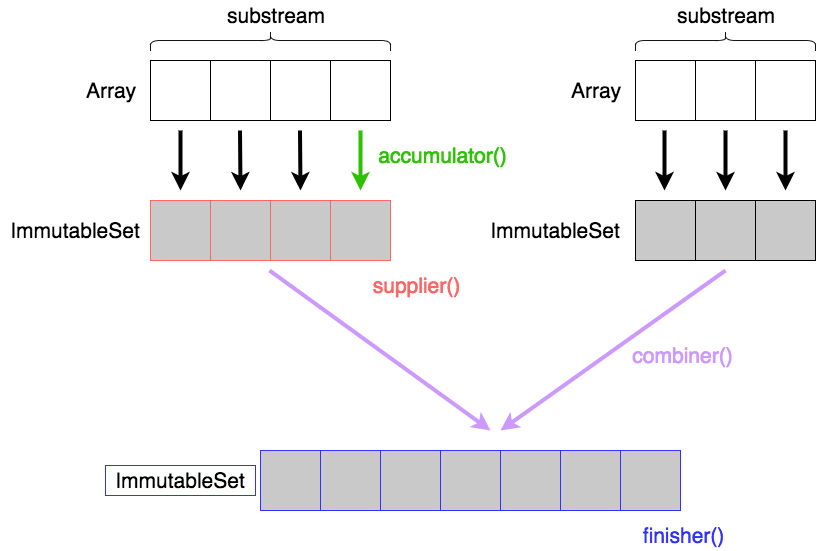
\includegraphics[width=13cm]{images/collector.png}
\caption{How a Collector is Used}
\source{Ethan Williams}
\label{fig:collector}
\end{figure}

The \verb|supplier()| method returns a mechanism to build an instance of a mutable data structure that will hold the elements of the stream which is known as the \textit{accumulator} \autocite{custom_collector}. Behind the scenes, the JVM will call this method several times to create \verb|ImmutableSet|s for all of the substreams \autocite{}.  In the code example our \verb|supplier()| is simply an \verb|ImmutableSet| builder so the JVM can generate new instances at will.

The \verb|accumulator()| method takes an accumulator and an element as parameters and will return a \verb|Consumer| object which details how the element should be added to the accumulator. The JVM uses this when of any element in the substream is done with processing to determine how or if it's added to the final data structure. In the code example, the \verb|accumulator| simply appends the element to the end of the \verb|ImmutableSet|.

The \verb|combiner()| method details the logic on how two accumulators should be joined together and is used to assemble all instances of the new data structure that were derived from substreams. In the code example the \verb|combiner()|'s behavior is that when two \verb|ImmutableSet|s are combined, one is simply appended to the other.

Finally, the \verb|finisher()| method serializes the accumulator that is the result of combining all the substreams, finishing the reduction. In the code example, this is as easy as returning the \verb|build()| method which serializes the \verb|ImmutableSet|, completing the conversion of the source.

\section{Practical Considerations when Using Parallel Streams}
Parallel streams were introduced to make implementing parallelism in a Java application easier, but with this ease comes common pitfalls that arise from the abstraction. For example, a common mistake is using long-running or blocking operations in a stream which is a bad concurrency practice to begin with. Additionally, many developers aren't familiar with interference and stateful expressions which can lead to severe errors in the application.

\subsection{Long-Running/Blocking Operations}
Using long-running or blocking operations in a stream will degrade performance drastically, a result of how streams implement threading. The JVM begins by processing on the calling thread and as more subtasks are broken off, the JVM gets threads from \verb|ForkJoinPool.common()|, which is a thread pool used in the background of the whole application \autocite{dzone_dangers}. 

With the JVM's use of a common thread pool, a long-running operation in a parallel stream as shown in the first example of Figure \ref{fig:network_op} will degrade performance drastically. Performance will be such that the stream will benefit very little from parallelization and may even be less performant than a serial stream. Each thread in the pool will be consumed executing that operation and subsequently all other JVM tasks using the common thread pool have to wait. 

In a situation where several streams are all attempting to process in parallel, each stream's performance will suffer even if it should have no problem. Java does allow a custom \verb|ThreadPool| like in example 2 of Figure \ref{fig:network_op} which can help by using threads created outside the common pool \autocite{dzone_fjp}. Unfortunately, since the issue described above results from a bad concurrency practice, more threads won't provide any significant performance enhancement.

\begin{figure}[H]
\centering
\begin{lstlisting}[language=Java]
// Example 1
Optional<String> result = collection.stream().parallel().map((base) -> longOperation(argument)).findAny();

// Example 2
ForkJoinPool customPool = new ForkJoinPool(4);
Optional<String> result = customPool.submit(() -> collection.stream().parallel().map((arg) -> longOperation(arg)).findAny()).get();
\end{lstlisting}
\caption{Reduction of employees into map by a Collector}
\source{Ethan Williams}
\label{fig:network_op}
\end{figure}

\begin{figure}[H]
\centering
\begin{lstlisting}[language=Java]

\end{lstlisting}
\caption{Reduction of employees into map by a Collector with custom Thread Pool}
\source{Ethan Williams}
\label{fig:custom_pool}
\end{figure}

\subsection{Interference}
Since \verb|Stream|s don't contain any of the elements of the collection, instead storing references, if the source is modified then the reference is invalidated \autocite{ibm_streams}. Editing the source of the stream in an intermediate operation is called \textit{interference} and will throw a \verb|ConcurrentModificationException| \autocite{parallelism_doc}. The stream in figure \ref{fig:interference} attempts to add each element to the collection again using the \verb|map()| method. Since it attempts to modify the source before the stream has serialized, this operation will throw an exception.

\begin{figure}[H]
\centering
\begin{lstlisting}[language=Java]
collection.stream().parallel().map((x) -> collection.add(x)).toArray();
\end{lstlisting}
\caption{A stream which causes interference and will throw an error}
\source{Ethan Williams}
\label{fig:interference}
\end{figure}

\subsection{Stateful Expressions} \label{stateful_expressions}
The third practice which will cause errors in a stream and should be watched carefully is using stateful expressions, which are operations that depends on the ordering of the elements \autocite{expression_state}. The code in Figure \ref{fig:stateful} shows an example of a stateful operation while attempting to add elements to \verb|parallelStorage| and print them. Although the \verb|forEachOrdered()| method is just fine and will print in the expected order, \verb|parallelStorage| will have a different ordering every time the stream is executed. The addition is stateful, meaning it depends on ordering and in parallel streams ordering can't be guaranteed in intermediate operations \autocite{parallelism_doc}.

\begin{figure}[H]
\centering
\begin{lstlisting}[language=Java]
List<String> parallelStorage = Collections.synchronizedList(new ArrayList<>());
collection.stream().parallel().map(x -> parallelSotrage.add(x)).forEachOrdered(x -> System.out.println(x));
\end{lstlisting}
\caption{A stream which causes interference and will throw an error}
\source{Ethan Williams}
\label{fig:stateful}
\end{figure}
 
\printbibliography[heading=bibintoc]

\appendix
\section{\\Code Example from Section 3.2}
\begin{figure}[H]
\centering
\begin{lstlisting}[language=Java]
import com.google.common.collect.ImmutableSet;
 
public class ImmutableSetCollector<T> 
        implements Collector<T, ImmutableSet.Builder<T>, ImmutableSet<T>> {
    @Override
    public Supplier<ImmutableSet.Builder<T>> supplier() {
        return ImmutableSet::builder;
    }
 
    @Override
    public BiConsumer<ImmutableSet.Builder<T>, T> accumulator() {
        return (builder, t) -> builder.add(t);
    }
 
    @Override
    public BinaryOperator<ImmutableSet.Builder<T>> combiner() {
        return (left, right) -> {
            left.addAll(right.build());
            return left;
        };
    }
 
    @Override
    public Function<ImmutableSet.Builder<T>, ImmutableSet<T>> finisher() {
        return ImmutableSet.Builder::build;
    }
}
\end{lstlisting}
\caption{Custom Collector }
\source{\autocite{custom_collector}}
\label{fig:collector_impl}
\end{figure}

\end{document}